\documentclass [a4paper] {article}
\usepackage[utf8]{inputenc}
\title{Ciencia de datos, práctica 2}
\author{Juan Casado Ballesteros, Samuel García Gonzalez, Iván Anaya Martín}
\usepackage{Sweave}
\begin{document}
\maketitle

\begin{abstract}
En este documento realizaremos anális de clasificación supervisada de cuatro muestras de datos propuestas por el profesor y cuatro muestras elegidas por nosotros.
La mitad de las muestras de cada tipo serán datos cuyo anális es realizable mediante árboles de clasificación de Hunt y la otra mitad por anális de regresión.

En el caso de los árboles de decisión de Hunt compareremos la clasificación atendiendo al criterio de maximización del incremeto de información
calculando esta mediante GINI y entropía comparando los resultado de utilizar una u otra métrica.
En esta parte (EJ1, EJ2 y las dos primeras muestras del EJ5) utilizaremos las librerías rpart, tree y party donde la función ctree nos permite crear los árboles de decisión.
Adicionalmente utilizaremos la librería rpart.plot como complemento de rpart para mostrar los árboles de decisión que esta librería genera.

En el anális de la regresión utilizaremos la función de R lm.
Adicionalmente hemos implementado nuestras propias funciones para el cálculo de regresión basadas en las fórmulas vistass en teoría.
Compararemos nuestros resultado con los de lm para comprobar que realizamos los cálculos correctamente y explicaremos por qué algunos de ellos difieren.

Las muestras proporcionadas se almecenarán en archivos .txt siendo esta de tamaño reducido.
Las muestras que nosotros hemos buscado en keaggle están en archivos .csv y tienen una cantidad de datos considerablemente mayor.
\end{abstract}

\newpage
\tableofcontents


%------------------------------------------------------------------------------------------------------------------------------------------------------------------------
\newpage
\section{EJ1}
Analizaremos los árboles de decisión mediante GINI y ENTROPÍA generados por rpart y tree para los datos de la muestra 1.
Los datos se componen de las calificaciones de distintos estudiantes en distintas pruebas y de la calificación final (Aprobado o Suspenso).
Predendemos averguar si se puede predecir la calificación final con menos pruebas.

Para los tres casos obtendremos el mismo árbol, los datos son reducidos y solo hay una solución posible en la que el incremento de la información se minimice.
Si hubiera más datos podríamos darse el caso de que se obtuviueran árboles distintos al utilizar GINI o entropía.
\begin{Schunk}
\begin{Sinput}
> muestra1 = data.frame(read.table("datos1.txt"))
> muestra1
\end{Sinput}
\begin{Soutput}
  Teoría Laboratorio Prácticas Global
1      A           A         B     AP
2      A           B         D     SS
3      D           D         C     SS
4      D           D         A     SS
5      B           C         B     SS
6      C           B         B     AP
7      B           B         A     AP
8      C           D         C     SS
9      B           A         C     SS
\end{Soutput}
\end{Schunk}

\newpage
\subsection{Rpart GINI}
\begin{center}
\begin{Schunk}
\begin{Sinput}
> clas_1gini=rpart(Global~., data=muestra1,method="class",minsplit=1)
> rpart.plot(clas_1gini)
\end{Sinput}
\end{Schunk}
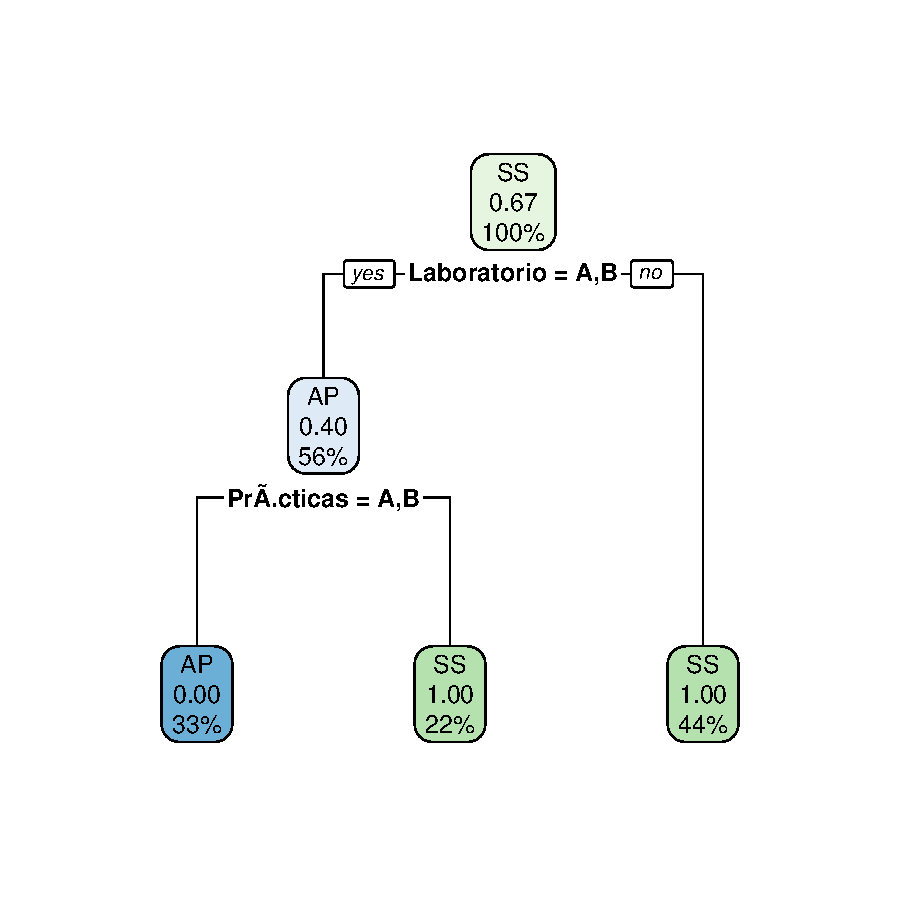
\includegraphics{entrega-rpart1_gini}
\end{center}

\newpage
\subsection{Rpart ENTROPÍA}
\begin{center}
\begin{Schunk}
\begin{Sinput}
> clas_1entropia=rpart(Global~., data=muestra1,method="class",minsplit=1,
+                       parms=list(split="information"))
> rpart.plot(clas_1entropia)
\end{Sinput}
\end{Schunk}
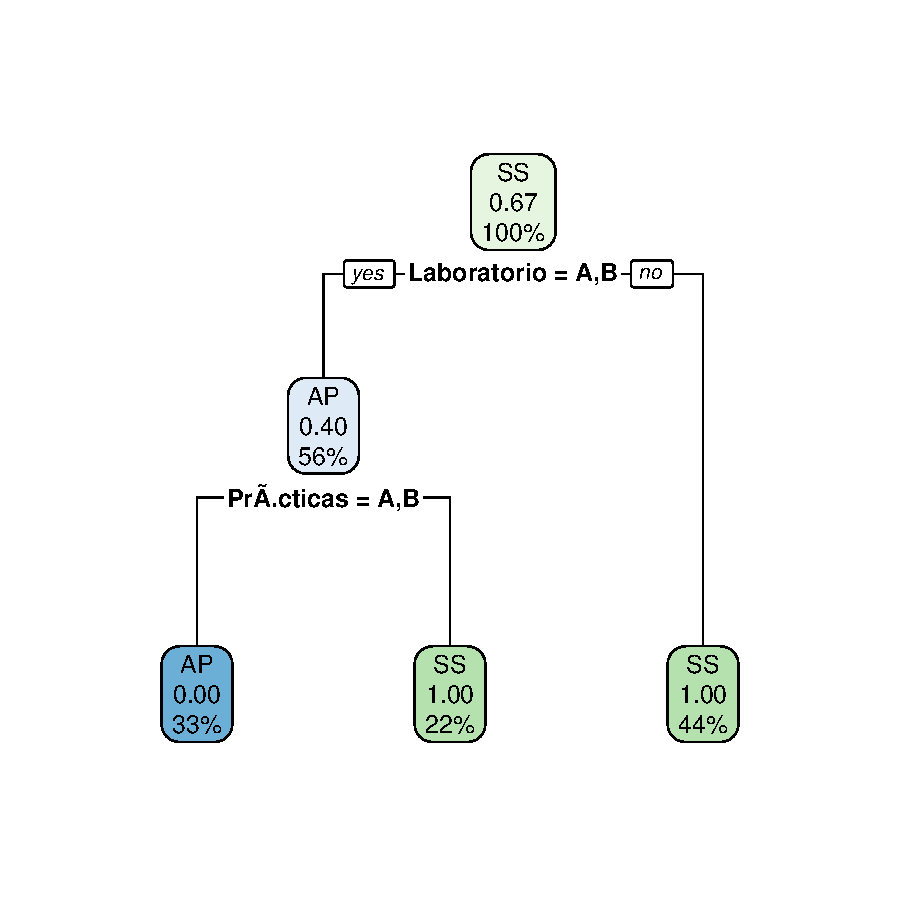
\includegraphics{entrega-rpart1_entropia}
\end{center}

\newpage
\subsection{Tree GINI}
\begin{center}
\begin{Schunk}
\begin{Sinput}
> clas_1tree=tree(Global~.,data=muestra1,mincut=1,minsize=2) 
> draw.tree(clas_1tree)
\end{Sinput}
\end{Schunk}
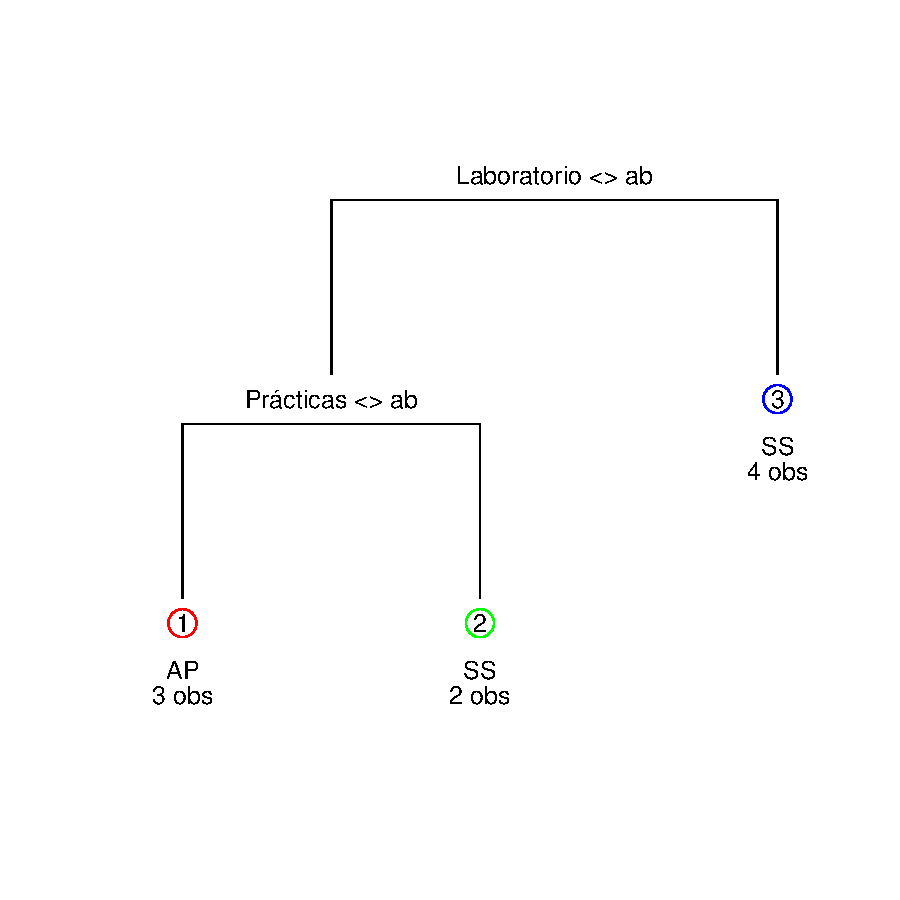
\includegraphics{entrega-tree1}
\end{center}

\subsection{Conclusiones}
Los árboles de decisión generados nos indican que para poder dilucidar si un alumno ha aprobado o no solo nos hace falta evaluar las notas de laboratorio y prácticas,
si en ambas han obtenido calificaciones de A o B podremos inferir que el alumno habrá aprobado si tener que considerar su nota de teoría.

%------------------------------------------------------------------------------------------------------------------------------------------------------------------------
\newpage
\section{EJ2}
Creamos un .txt con los datos proporcionados sobre el radio y densidad de los planetas y lo leemos.
\begin{Schunk}
\begin{Sinput}
> datos2 <- read.table("datos2.txt")
> datos2
\end{Sinput}
\begin{Soutput}
    Nombre Radio Densidad
1 Mercurio   2.4      5.4
2    Venus   6.1      5.2
3   Tierra   6.4      5.5
4    Marte   3.4      3.9
\end{Soutput}
\end{Schunk}

\subsection{Cálculo de la recta de regresión}
Calculamos la regresión sobre dichos datos para obtener la recta que más se aproxime a los puntos que tenemos.
\begin{Schunk}
\begin{Sinput}
> regresion2 <- lm(Densidad~Radio, data=datos2)
> regresion2_own <- regLine(datos2$Radio, datos2$Densidad)
\end{Sinput}
\end{Schunk}

Podemos ver los valores que adopta la ecucaión de la recta que se generará.

\begin{Schunk}
\begin{Soutput}
[1] "y = 0.139366900361164 * x + 4.36239643084768"
\end{Soutput}
\begin{Soutput}
[1] "y = 0.139366900361164 * x + 4.36239643084767"
\end{Soutput}
\end{Schunk}

\subsection{Análisis de la regresión}
Cuando calculamos la recta de regresión sobre unos datos es necesario evaluar la calidad de esta.
Debemos analizar cómo de bien se ajusta a nuestros datos.
Podemos ver esta información mediante summary.

\subsubsection{Residuos}
Diferencias entre cada valor de y real y cada valor de y obtenido mediante la función de regresión.
\begin{Schunk}
\begin{Sinput}
> summary(regresion2)$residuals
\end{Sinput}
\begin{Soutput}
          1           2           3           4 
 0.70312301 -0.01253452  0.24565541 -0.93624389 
\end{Soutput}
\end{Schunk}

\subsubsection{Coeficientes}
Coeficientes estimados para y error estándar para cada uno de ellos.
\begin{Schunk}
\begin{Sinput}
> summary(regresion2)$coefficients
\end{Sinput}
\begin{Soutput}
             Estimate Std. Error   t value   Pr(>|t|)
(Intercept) 4.3623964  1.2049754 3.6203201 0.06854492
Radio       0.1393669  0.2466205 0.5651067 0.62893696
\end{Soutput}
\end{Schunk}

\subsubsection{Error estándar}
R implemnta el error estándar de la población y no el de la muestra que el que hemos visto en clase por lo que los cálculos no coincidirán.
El error estándar de la población se divide por n-2 y el de la muestra solo por n.
Cuanto más próximo a 0 sea el error estándar mejor será la recta de regresión.
\begin{Schunk}
\begin{Sinput}
> summary(regresion2)$sigma
\end{Sinput}
\begin{Soutput}
[1] 0.8460019
\end{Soutput}
\begin{Sinput}
> errorEstandar(datos2$Radio, datos2$Densidad, regresion2_own)
\end{Sinput}
\begin{Soutput}
    Radio 
0.5982136 
\end{Soutput}
\end{Schunk}

\subsubsection{Correlación cuadrada}
Podemos comprobar que coincide con nuestra implementación.
Este valor está entre 0 y 1 siendo mejor cuanto más próximo a 1 sea (idealmente a partir de 0.8).
\begin{Schunk}
\begin{Sinput}
> summary(regresion2)$r.squared
\end{Sinput}
\begin{Soutput}
[1] 0.1376878
\end{Soutput}
\begin{Sinput}
> correlacionCuadrada(datos2$Radio, datos2$Densidad, regresion2_own)
\end{Sinput}
\begin{Soutput}
[1] 0.1376878
\end{Soutput}
\end{Schunk}

\subsection{Visualización de la recta de regresión}
Para finalizar dibujaremos una gráfica en la que se representarán lod datos junto a la recta de regresión.
Paralela a la recta de regresión dibujaremos las rectas que marcan el error estándar entorno a la recta de regresión.
En trazado gris grueso la que marca la región en la que estarán el 66\% de los datos y en gris fino la que marca el 95\%.
\begin{center}
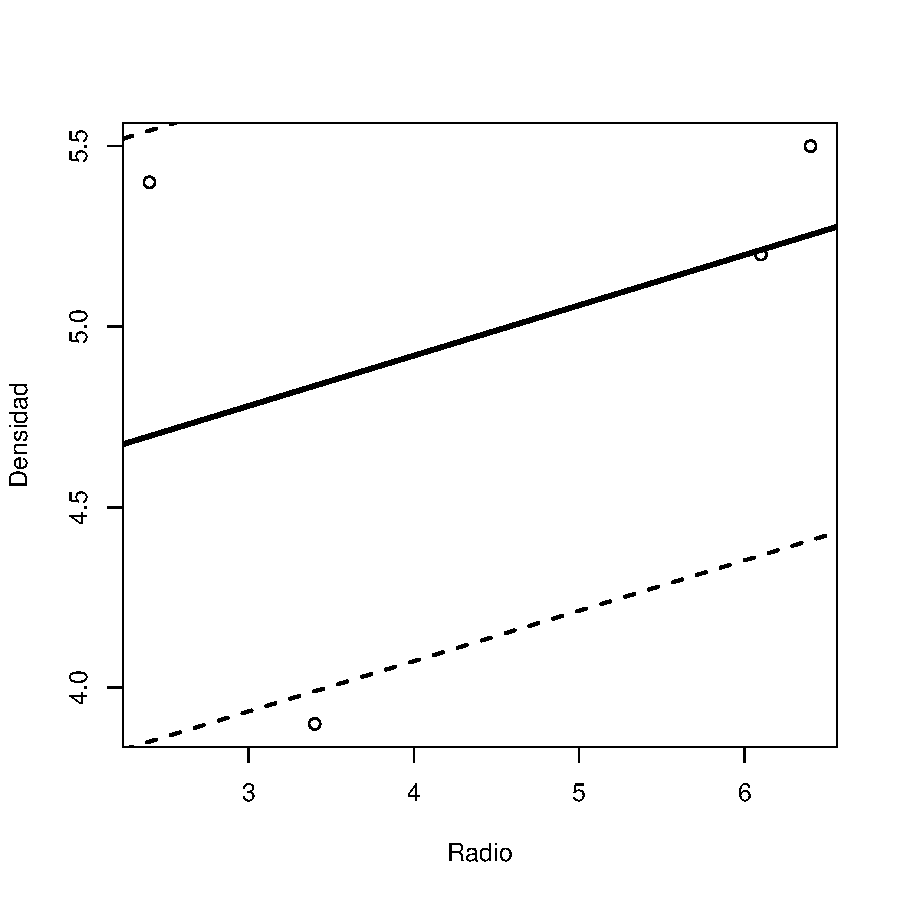
\includegraphics{entrega-plot_regresion2}
\end{center}

Como podemos ver la recta se ajusta muy mal a los datos que tenemos quedando las rectas que marcan el error estandas fuera del gráfico.
La correlación cuadrada obtenida es muy baja.
En parte esto se debe a que tenemos muy pocos datos.

%------------------------------------------------------------------------------------------------------------------------------------------------------------------------
\newpage
\section{EJ3}
En esta parte realizamos el algoritmo Hunt con la librería rpart sobre los datos de los vehículos.
Lo primero sera realizar el ejercicio usando Gini como metodo para calculart la impureza.
La segunda parte la calcularemos usando la entropia. 
Por último utilizaremos la libreria tree para repetir estos cálculos aunque solo podremos utilizar Gini para calcular la impuraza.
En ambos casos mostraremos los árboles obtenidos con las librerías adecuadas.
\begin{Schunk}
\begin{Sinput}
> muestra3 = data.frame(read.table("datos3.txt"))
> muestra3
\end{Sinput}
\begin{Soutput}
   TipoCarnet NumeroRuedas NumeroPasajeros TipoVehiculo
1           B            4               5        Coche
2           A            2               2         Moto
3           N            2               1    Bicicleta
4           B            6               4       Camion
5           B            4               6        Coche
6           B            4               4        Coche
7           N            2               2    Bicicleta
8           B            2               1         Moto
9           B            6               2       Camion
10          N            2               1    Bicicleta
\end{Soutput}
\end{Schunk}

\newpage
\subsection{Rpart GINI}
\begin{center}
\begin{Schunk}
\begin{Sinput}
> clas_3gini=rpart(TipoVehiculo~., data=muestra3,method="class",minsplit=1)
> rpart.plot(clas_3gini)
\end{Sinput}
\end{Schunk}
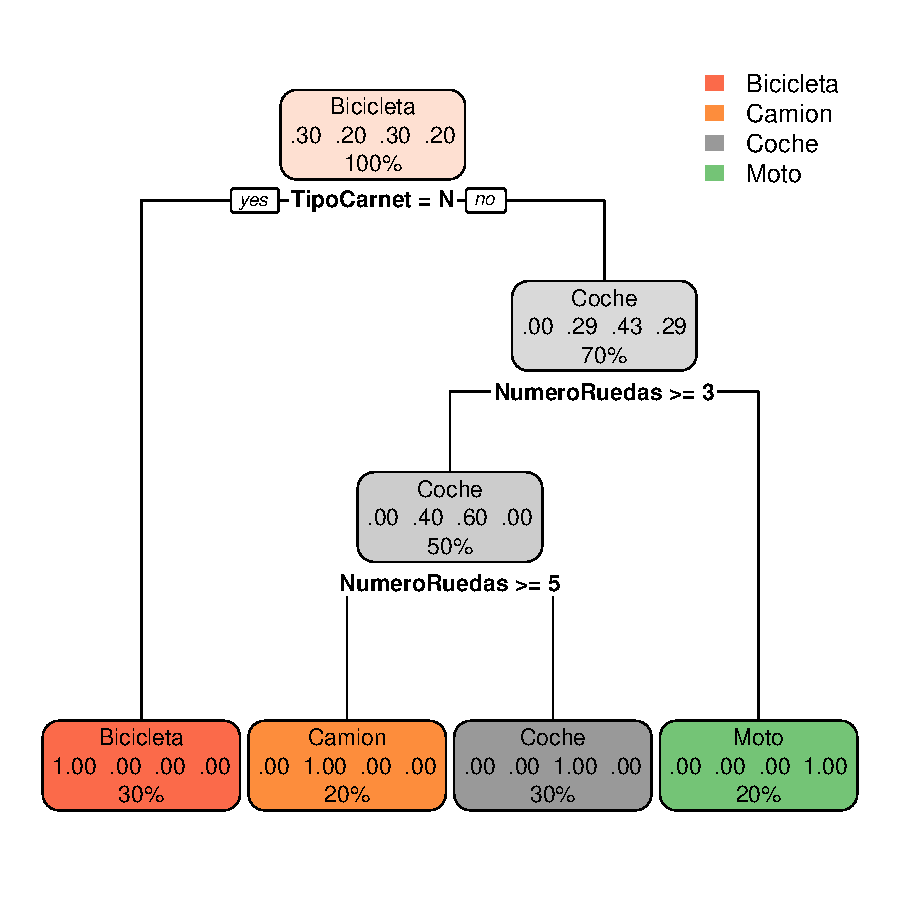
\includegraphics{entrega-rpart3_gini}
\end{center}

\newpage
\subsection{Rpart ENTROPÍA}
Ahora utilizaemos la entropia. 
Para ello añadimos el parametro parms=list(split="information").
Por defecto esta se clasifica por Gini.
\begin{center}
\begin{Schunk}
\begin{Sinput}
> clas_3entropia=rpart(TipoVehiculo~., data=muestra3,method="class",minsplit=1,
+                       parms=list(split="information"))
> rpart.plot(clas_3entropia)
\end{Sinput}
\end{Schunk}
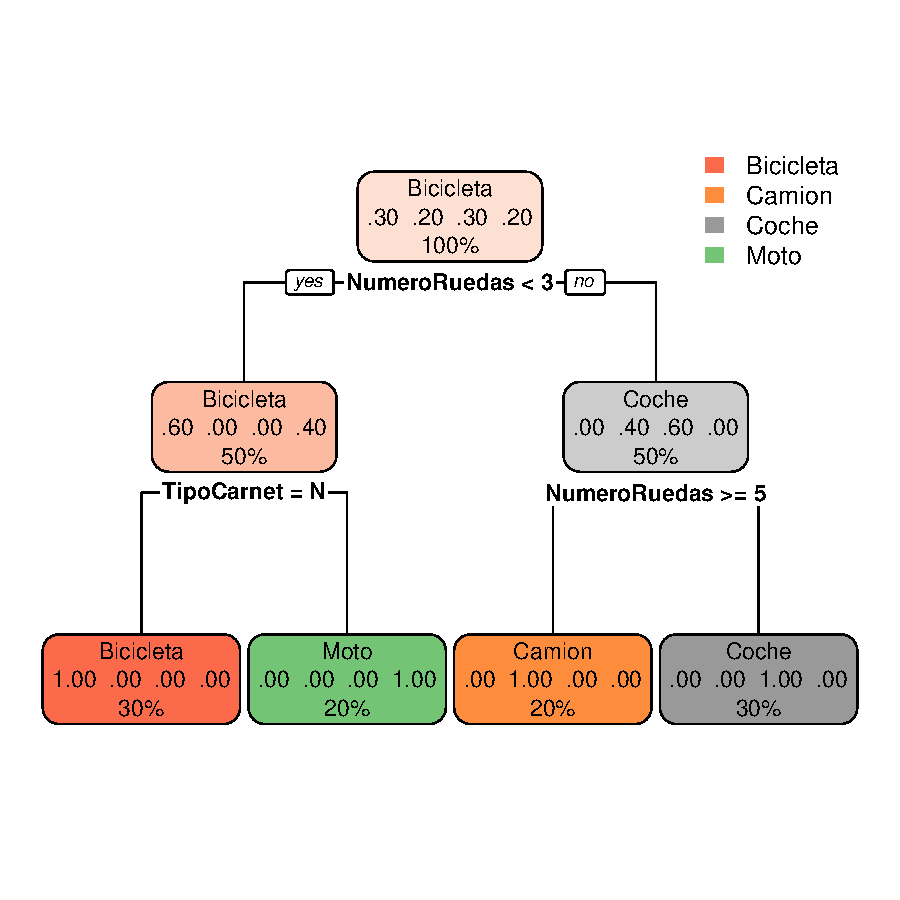
\includegraphics{entrega-rpart3_entropia}
\end{center}

Vemos que el árbol obtenido es distinto.
En el caso del arbol obtenido con Gini la profundidad es 3 mientras que en el obtenido con Entropia es de 2.
Cuando utilizamos Gini para generar los árboles estos tienden a tener una rama muy oprofunda de la que cuelgan otras de profundidad relativa de 2.
Dependiendo del tipo de árbol que queramos generar será recomendable utilizar una medida de información u otra.

\newpage
\subsection{Tree GINI}
Ahora realizamremos los mismo cálculos con tree.
\begin{center}
\begin{Schunk}
\begin{Sinput}
> clas_3tree=tree(TipoVehiculo~.,data=muestra3,mincut=1,minsize=2) 
> draw.tree(clas_3tree)
\end{Sinput}
\end{Schunk}
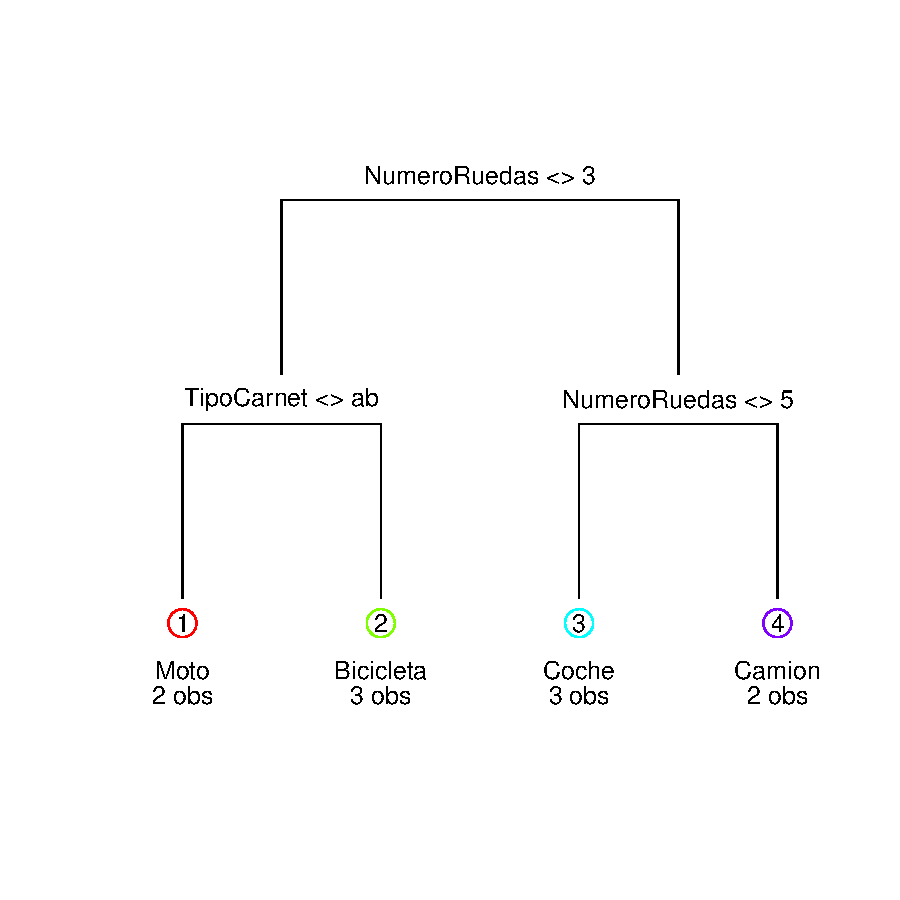
\includegraphics{entrega-tree3}
\end{center}

El arbol generado es igual que el obtenido con rpart con aplicando gini.
Ya que por defecto tree implementa el gini.
En esta libreria no esta implentado el calculo por entropia.

\subsection{Conclusiones}
En este caso podremos ver que obtenemos dos árboles de decisión distintos pero igualmente válidos.
Si no tenemos carnet tendremos una bicicleta,
si tenemos carnet y menos de tres ruedas una moto,
si tenemos más de cinco ruedas tendremos un camión y
si tenemos cuatro ruedas tendremos un coche.


%------------------------------------------------------------------------------------------------------------------------------------------------------------------------
\newpage
\section{EJ4}
Realizaremos un anális de regresión lineal de los datos de las 4 muestras proporcionadas.
Al igual que en el EJ2 utilizaremos la función lm y compararemos los resultados de esta con los obtenidos por las funciones que hemos implementado nosotros.
Comenzamos por cargar los datos del fichero .txt.
\begin{Schunk}
\begin{Sinput}
> datos4 <- read.table("datos4.txt")
> datos4
\end{Sinput}
\begin{Soutput}
   x1    y1 x2   y2 x3    y3 x4    y4
1  10  8.04 10 9.14 10  7.46  8  6.58
2   8  6.95  8 8.14  8  6.77  8  5.76
3  13  7.58 13 8.74 13 12.74  8  7.71
4   9  8.81  9 8.77  9  7.11  8  8.84
5  11  8.33 11 9.26 11  7.81  8  8.47
6  14  9.96 14 8.10 14  8.84  8  7.04
7   6  7.24  6 6.13  6  6.08  8  5.25
8   4  4.26  4 3.10  4  5.39 19 12.50
9  12 10.84 12 9.13 12  8.15  8  5.56
10  7  4.82  7 7.26  7  6.42  8  7.91
11  5  5.68  5 4.74  5  5.73  8  6.89
\end{Soutput}
\end{Schunk}
\subsection{Cálculo de las rectas de regresión}
Utilizando lm y nuestra función propia obtenemos las rectas de regresión que serán 4 rectas, una para cada muestra.
\begin{Schunk}
\begin{Sinput}
> regresion41 <- lm(y1~x1, data=datos4)
> regresion41_own <- regLine(datos4$x1, datos4$y1)
> regresion42 <- lm(y2~x2, data=datos4)
> regresion42_own <- regLine(datos4$x2, datos4$y2)
> regresion43 <- lm(y3~x3, data=datos4)
> regresion43_own <- regLine(datos4$x3, datos4$y3)
> regresion44 <- lm(y4~x4, data=datos4)
> regresion44_own <- regLine(datos4$x4, datos4$y4)
\end{Sinput}
\end{Schunk}

Podemos ver como la pendiente de todas las recta y su intersección con el origen es muy similar.
Las recta de regresión obtenidas para cada muestra se parecerán mucho.
\begin{Schunk}
\begin{Soutput}
[1] "y1 = 0.500090909090909 * x1 + 3.00009090909091"
\end{Soutput}
\begin{Soutput}
[1] "y1 = 0.500090909090908 * x1 + 3.00009090909092"
\end{Soutput}
\begin{Soutput}
[1] "y2 = 0.500090909090909 * x2 + 3.00009090909091"
\end{Soutput}
\begin{Soutput}
[1] "y2 = 0.500090909090908 * x2 + 3.00009090909092"
\end{Soutput}
\begin{Soutput}
[1] "y3 = 0.500090909090909 * x3 + 3.00009090909091"
\end{Soutput}
\begin{Soutput}
[1] "y3 = 0.500090909090908 * x3 + 3.00009090909092"
\end{Soutput}
\begin{Soutput}
[1] "y4 = 0.500090909090909 * x4 + 3.00009090909091"
\end{Soutput}
\begin{Soutput}
[1] "y4 = 0.500090909090908 * x4 + 3.00009090909092"
\end{Soutput}
\end{Schunk}

\subsection{Análisis de la regresión}
Analizaremos ahora lo bien o mal que se ajusta cada recta a los datos a partir los que se creó.

\subsubsection{Error estándar}
Podemos ver que el error estándar es alto, podría estar mucho más próximo a 0.
La recta de regresión no es especialmente buena.
El error obtenido para todas las recta es aproximadamente el mismo.
\begin{Schunk}
\begin{Soutput}
[1] "Error estándar de la población 1: 1.23660332272632 y de la muestra 1: 2.47034838909454"
\end{Soutput}
\begin{Soutput}
[1] "Error estándar de la población 2: 1.23721420534158 y de la muestra 2: 2.47046591366761"
\end{Soutput}
\begin{Soutput}
[1] "Error estándar de la población 3: 1.23631135139 y de la muestra 3: 2.46900451270313"
\end{Soutput}
\begin{Soutput}
[1] "Error estándar de la población 4: 1.23569548568138 y de la muestra 4: 2.46971119906276"
\end{Soutput}
\end{Schunk}

\subsubsection{Correlación cuadrada}
Al igual que hemos visto con el error estardar, la correlación no es muy buena, es ente caso por no estar sufic iéntemente próximas a 1.
Las rectas de regresión obtenidas no son de calidad, no se ajustan bien a los datos.
\begin{Schunk}
\begin{Soutput}
[1] "Calculada con lm 1: 0.666542459508775 y calculada por nosotros 1: 0.666542459508771"
\end{Soutput}
\begin{Soutput}
[1] "Calculada con lm 2: 0.666242033727484 y calculada por nosotros 2: 0.666242033727484"
\end{Soutput}
\begin{Soutput}
[1] "Calculada con lm 3: 0.666324041066559 y calculada por nosotros 3: 0.666324041066552"
\end{Soutput}
\begin{Soutput}
[1] "Calculada con lm 4: 0.666707256898465 y calculada por nosotros 4: 0.666707256898469"
\end{Soutput}
\end{Schunk}

\subsection{Visualización de las rectas de regresión}
Dibujaremos ahora cada recta junto a las líneas que marcan las regiones en las que se deben encontrar al menos el 66\% de los datos y en gris fino la que marca el 95\%.
Podemos ver las que rectas son muy similares, ninguna se ajusta bien a los datos.
Los datos son de naturaleza muy distinta.

Los primeros datos son muy dispersos,
la relación en los segundos no es lineal,
en el tercer caso hay un dato anómalo que "estropea" la regresión y
en el último caso los datos no parecen estar relacionados con la resta si no fuera por el último valor que también es anómalo.
\begin{center}
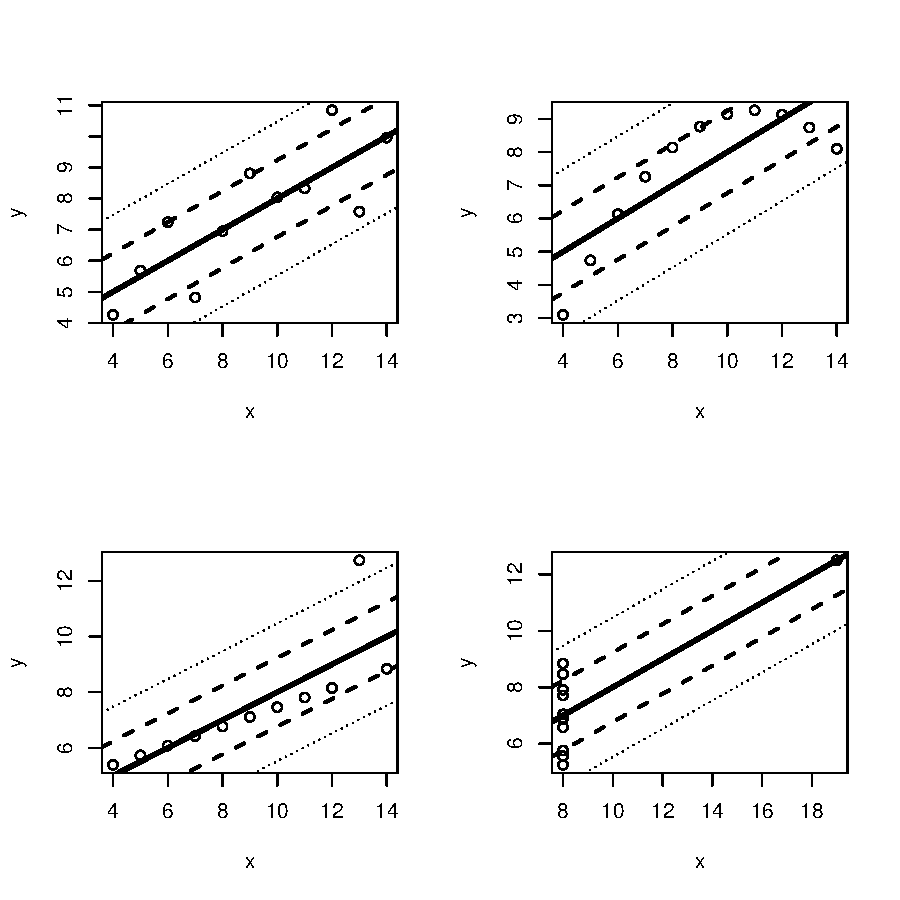
\includegraphics{entrega-plot_regresion4}
\end{center}
El orden en el que se han analizado las gráficas es el [1,1]; [1,2]; [2,1]; [2,2] primero en horizonal y luego en vertical.

%------------------------------------------------------------------------------------------------------------------------------------------------------------------------
\newpage
\section{EJ5}
Para este último ejecrcicio hemos tomado cuatro muestras de la página de keaggle y analizaremos cada una de ellas mediante árboles de decisión de Hunt
o mediante regresión según sea más conveniente por la naturaleza de los datos.
Todos los datos analizados se encuentran en formato .csv

\subsection{Análisis de los datos de un banco pra decidir si conceder créditos o no a sus clientes}
Los datos se han obtenido de https://www.kaggle.com/ajay1735/hmeq-data.
En este caso el árbol de decisión nos genera hojas en las que se indica la probabilidad de que a un cliente se le deba conceder o no un crédito.
Vemos que de las 12 varibales consideradas en los datos de entrada para decidirlo en el árbol solo se utilizan 8 teniendo que hacer en el peor caso 7 comprobaciones y 4 en el mejor.

En en dos nodos donde se centra la mayor cantidad de gente a la que no se le be conceder,
si tienen alguna línea de crédito con deudas y
tinen un ratio de deuda respecto a ingresos mayor del 46\% y
el crédito que piden supera los 5050 dólares así como
si no tienen menos de cinco líneas de crédito endeudadas
con más de cuatro líneas de crédito solicitadas recientemente y
su ratio de rentas e ingresos en menor del 44\% y
ha pedido más de 6050 dólares de crédito y
tienen menos de 3 prórrogas de pago y
la línea de crédito más antigua es de más de 76 meses.

Hay otros dos nodos donde tampoco es recomdable dar crédito pero en estos hay clasificada menos gente.
Es sorprendente que el porcentaje de gente a la que se le deba dar crádito es muy bajo.
\begin{Schunk}
\begin{Sinput}
> bank <- read.csv("hmeq.csv")
> bank <- data.frame(bank, method="class", minsplit=1)
\end{Sinput}
\end{Schunk}
\begin{center}
\begin{Schunk}
\begin{Sinput}
> cls_bank_rpart <- rpart(BAD~., data=bank, method="class", minsplit=1)
> rpart.plot(cls_bank_rpart, box.palette="RdBu", shadow.col="gray", nn=TRUE)
\end{Sinput}
\end{Schunk}
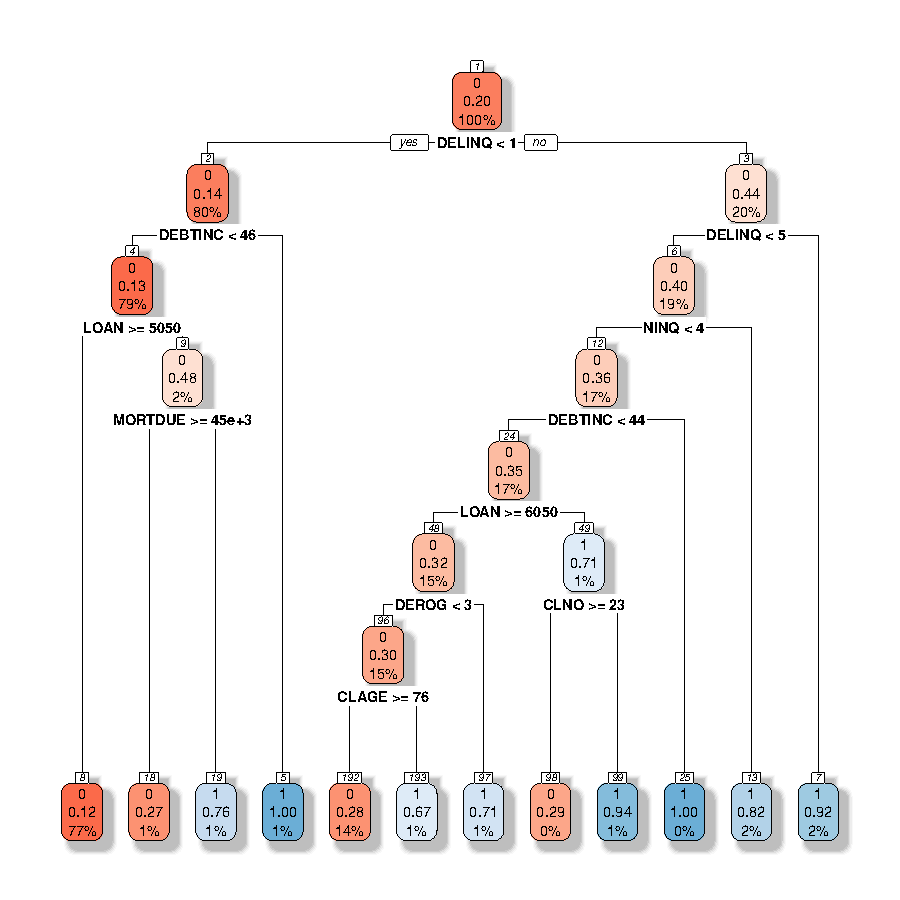
\includegraphics{entrega-analisis_banco_rpart}
\begin{Schunk}
\begin{Sinput}
> cls_bank_ctree <- ctree(BAD~., data=bank)
> plot(cls_bank_ctree)
\end{Sinput}
\end{Schunk}
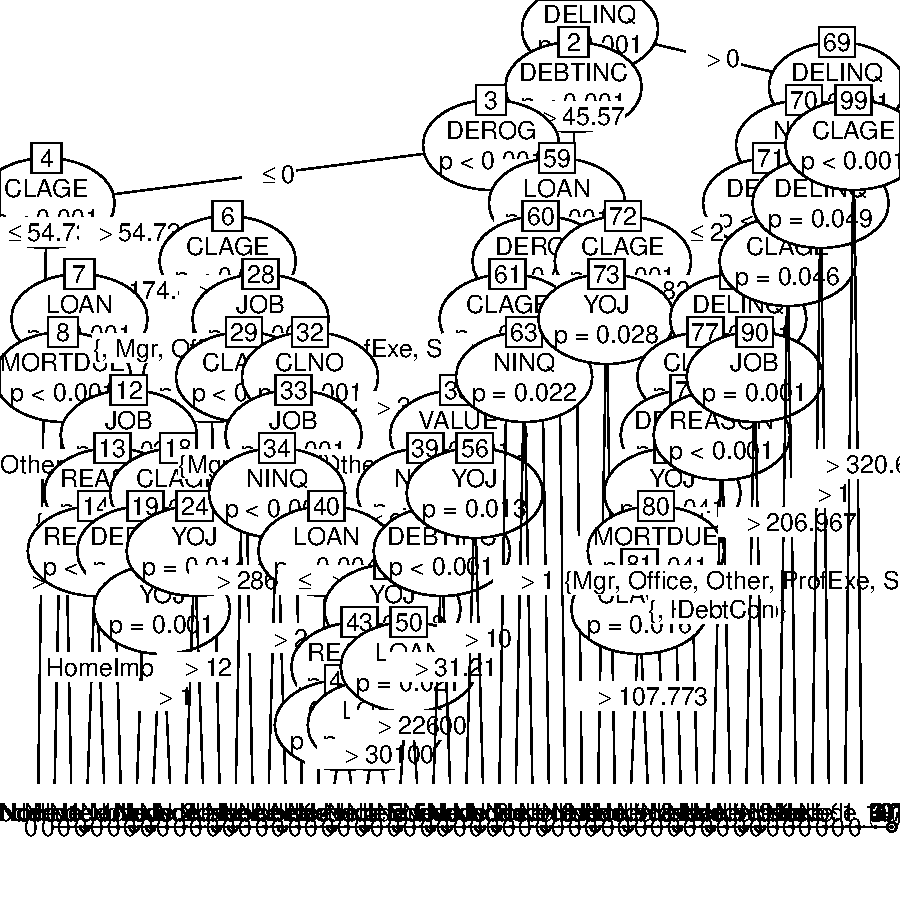
\includegraphics{entrega-analisis_banco_ctree}
\end{center}
Podemos ver que las capacidades de rpart para visualizar los datos de modo inteligible son mayores que las de la librería party.
En el árbol dibujado con esta librería es difícil verlo.

\subsection{Análisis del juego de las tres en raya}
Los datos se obtuvieron de https://www.kaggle.com/aungpyaeap/tictactoe-endgame-dataset-uci.
En este caso analizaremos el fin de partidas de tres en raya para determinar cuando un jugador gana o pierde.
El árbol nos proporciona las probabilidades de que cada suceso ocurra en función de las posiciones de las piezas en el tablero.
Vemos que tendremos posibilidades de ganar cuando las piezas del rival están en ciertas casillas que no cortan que nosotros podamos hacer 3 en raya.
Es sorprendente que el a´rbol de decisión se genere entorno a este hecho en vez de mostrarnos las casillas en las que nosotros hacemos en tres en raya.
Esto se debe a que el número de casillas que nos cortan un tres en raya es inferior al casillas desde las que nosotoros podemos hacerlo.
También en elagunos casos se considera que algunas casillas no tengan ficha (b).
\begin{Schunk}
\begin{Sinput}
> game <- read.csv("tic-tac-toe-endgame.csv")
> game <- data.frame(game)
\end{Sinput}
\end{Schunk}
\begin{center}
\begin{Schunk}
\begin{Sinput}
> cls_game_rpart <- rpart(V10~., data=game, method="class", minsplit=1)
> rpart.plot(cls_game_rpart, box.palette="RdBu", shadow.col="gray", nn=TRUE)
\end{Sinput}
\end{Schunk}
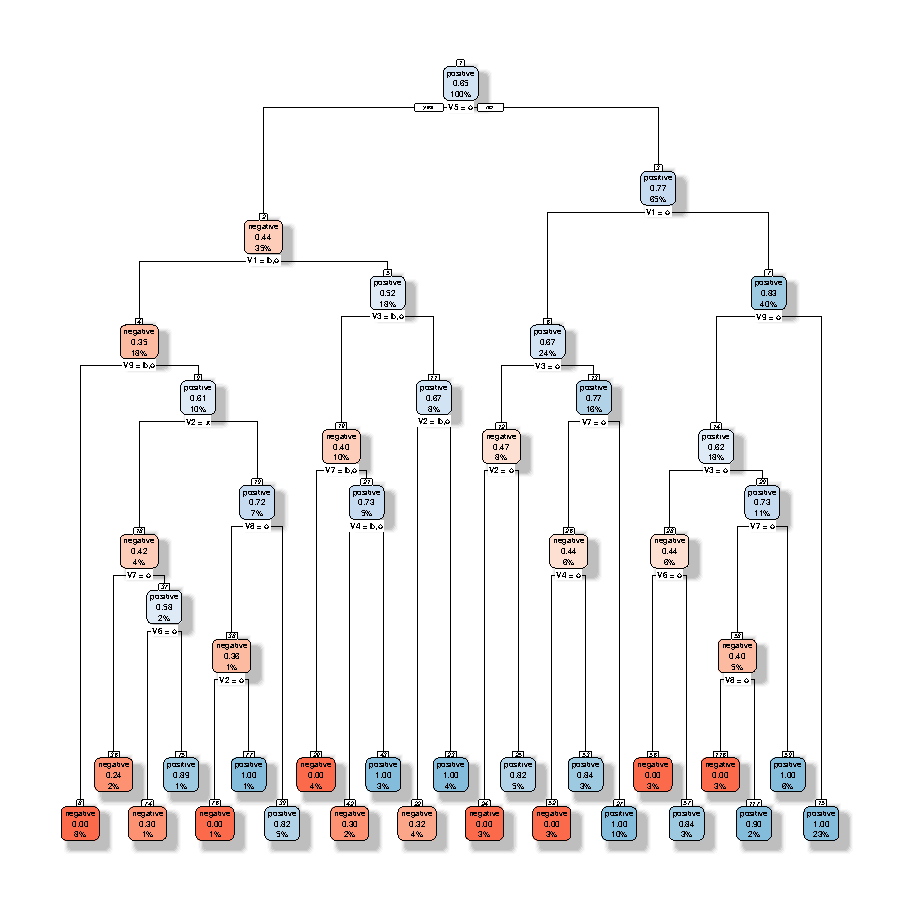
\includegraphics{entrega-analisis_juego_rpart}
\begin{Schunk}
\begin{Sinput}
> cls_game_ctree <- ctree(V10~., data=game)
> plot(cls_game_ctree)
\end{Sinput}
\end{Schunk}
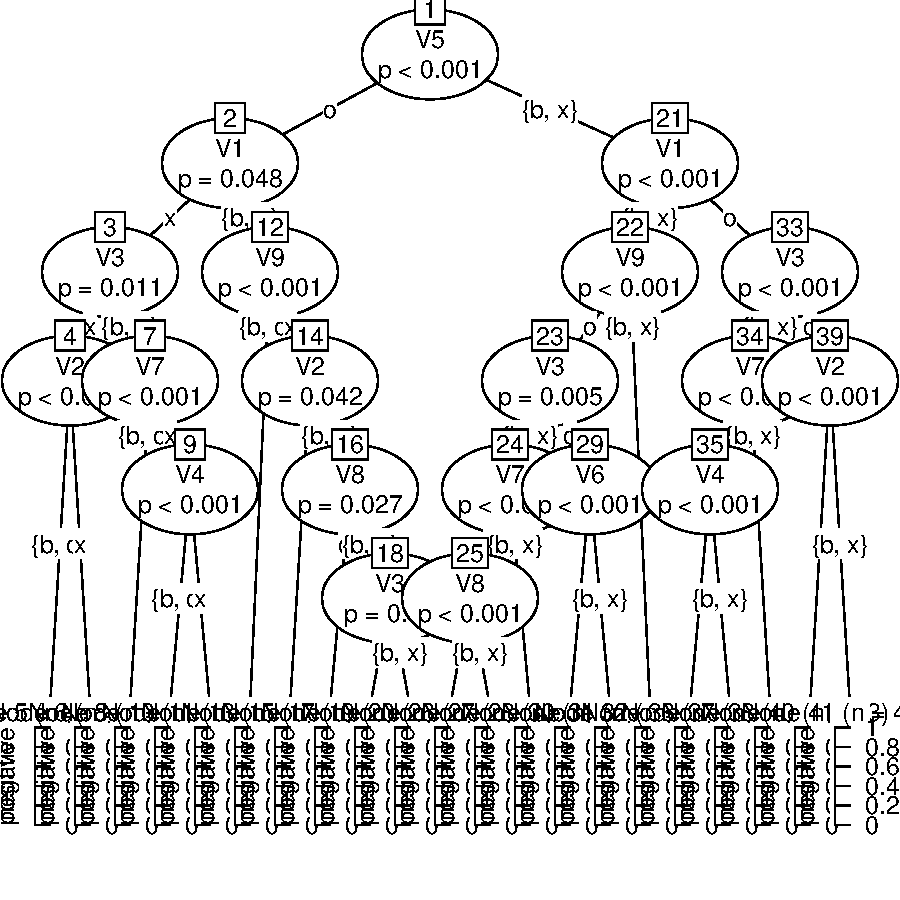
\includegraphics{entrega-analisis_juego_ctree}
\end{center}
Comprobamos una vez que el árbol generado por party es difícil de entender mientras que en el generado por rpart podemos hacerlo sin problemas.

\subsection{Análisis de los componente del cemento respecto de la resistencia de este}
Hemos tomado estos datos de https://www.kaggle.com/maajdl/yeh-concret-data.
Los datos representan la resistencia del hormigón respecto a la cantidad de distintas sustancias de las que este está compuesto.
\begin{Schunk}
\begin{Sinput}
> concrete <- read.csv("compresive_strength_concrete.csv")
> regresion_water <- lm(Water~Strength, data=concrete)
> regresion_cement <- lm(Cement~Strength, data=concrete)
> regresion_blast <- lm(Blast~Strength, data=concrete)
> regresion_ash <- lm(FlyAsh~Strength, data=concrete)
> regresion_plast <- lm(Superplasticizer~Strength, data=concrete)
> regresion_coarse <- lm(Coarse~Strength, data=concrete)
> regresion_fine <- lm(Fine~Strength, data=concrete)
> regresion_age <- lm(Age~Strength, data=concrete)
\end{Sinput}
\end{Schunk}
Vemos que la correlación cuadrada entre cada variable y la resistencia del hormigón es baja en todos los casos.
Ninguna variable considerada tiene relación directa con la resistencia final del hormigón.
En este caso esto se debe a que la relación de las varibales con la resistencia del hormigón no es lineal y que adimás es multidimensional.
\begin{Schunk}
\begin{Soutput}
[1] "Correlación cuadrada Water: 0.083887497698046"
\end{Soutput}
\begin{Soutput}
[1] "Correlación cuadrada Cement: 0.247836619897972"
\end{Soutput}
\begin{Soutput}
[1] "Correlación cuadrada Blast: 0.0181789297559356"
\end{Soutput}
\begin{Soutput}
[1] "Correlación cuadrada FlyAsh: 0.0111841023210516"
\end{Soutput}
\begin{Soutput}
[1] "Correlación cuadrada Superplasticizer: 0.134013707715721"
\end{Soutput}
\begin{Soutput}
[1] "Correlación cuadrada Coarse: 0.027203427047105"
\end{Soutput}
\begin{Soutput}
[1] "Correlación cuadrada Fine: 0.0279696347951344"
\end{Soutput}
\begin{Soutput}
[1] "Correlación cuadrada Age: 0.108157450642031"
\end{Soutput}
\end{Schunk}
Pueden observarse tendencias como que si hay demsiada agua o demasiado agregado fino la resistenci de este será baja (rectas con pendiente negativa).
\begin{center}
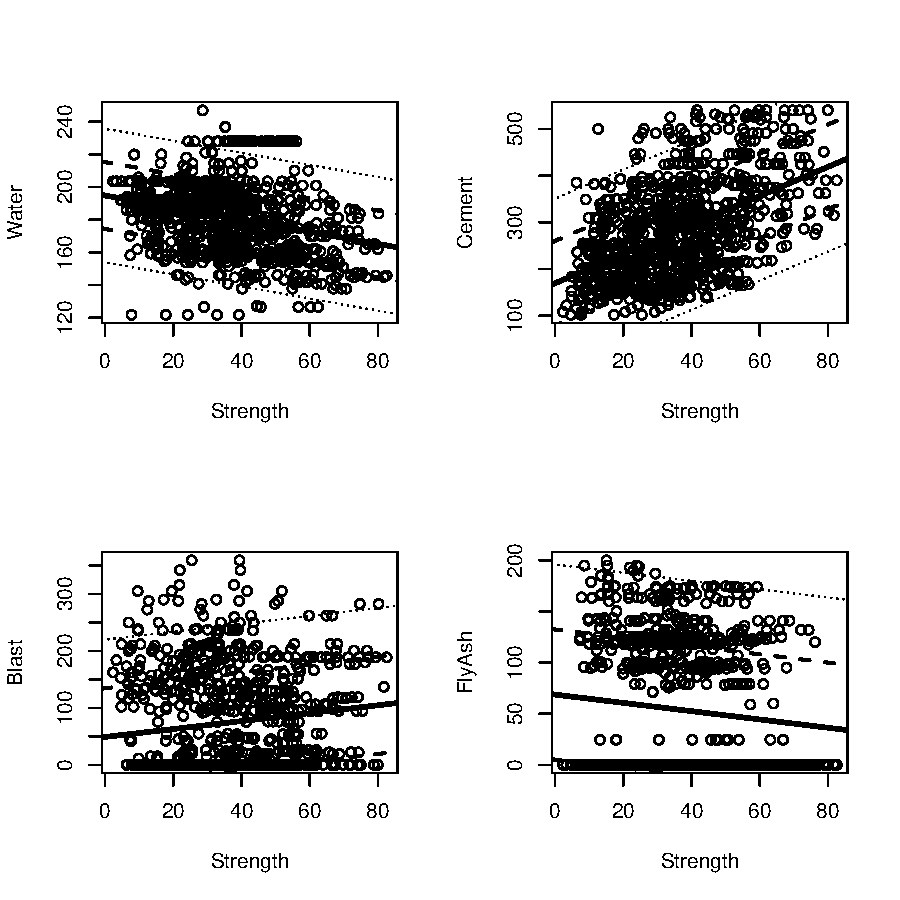
\includegraphics{entrega-analisis_concrete_plot_1}
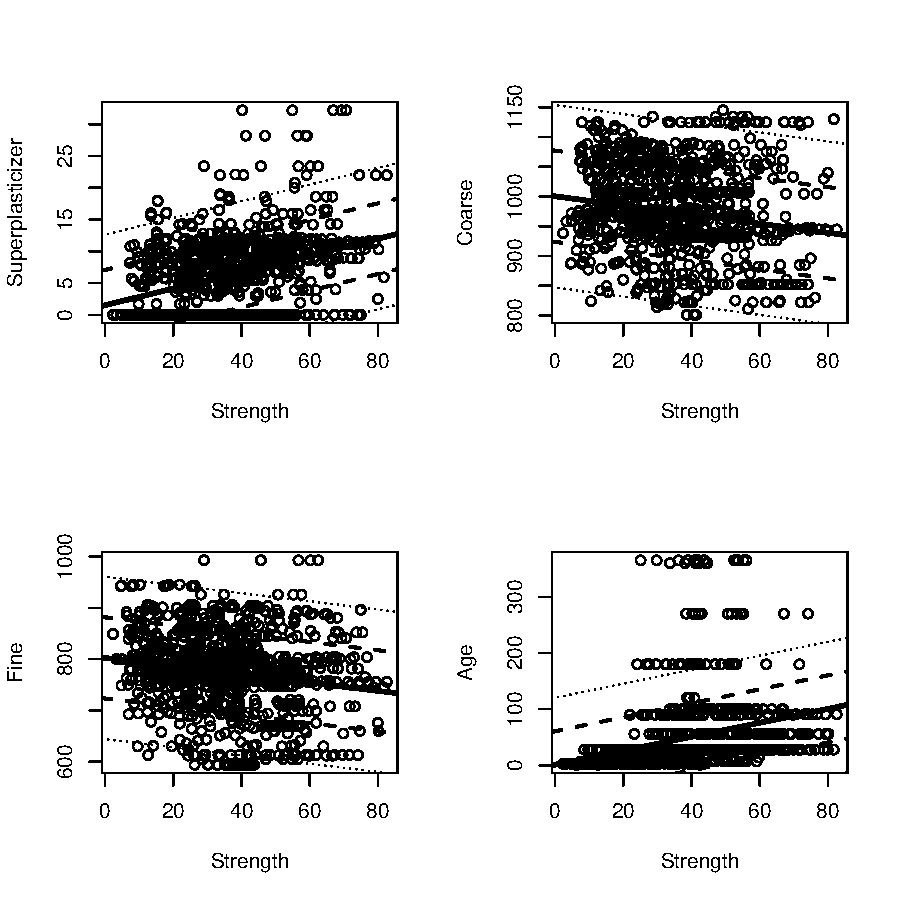
\includegraphics{entrega-analisis_concrete_plot_2}
\end{center}

\subsection{Análisis de las notas de alumnos respecto de su probabilidad de ser admitidos en la universidad}
Los datos fueron obtenidos de https://www.kaggle.com/mohansacharya/graduate-admissions.
La muestra representa las notas obtenidas en distintos exámenes con la probabilidad de admisión.
\begin{Schunk}
\begin{Sinput}
> grades <- read.csv("Admission_Predict.csv")
> regresion_gre <- lm(GRE~Admit, data=grades)
> regresion_toefel <- lm(TOEFL~Admit, data=grades)
> regresion_rating <- lm(UniversityRating~Admit, data=grades)
> regresion_sop <- lm(SOP~Admit, data=grades)
> regresion_lor <- lm(LOR~Admit, data=grades)
> regresion_research <- lm(Research~Admit, data=grades)
> regresion_cgpa <- lm(CGPA~Admit, data=grades)
\end{Sinput}
\end{Schunk}
En este caso podemos ver como las notas de los exámenes TOEFL y GRE así como la nota media del expediente tienen gran relación con la probabilidad de admisión.
En el resto de casos la correlación cuadrada es mucho menor.
La que más relacionada está es la nota media del expediente y la que menos es si el estudiante a realizado investigaciones o no.
\begin{Schunk}
\begin{Soutput}
[1] "Correlación cuadrada GRE: 0.644183549843835"
\end{Soutput}
\begin{Soutput}
[1] "Correlación cuadrada TOEFL: 0.626621040151816"
\end{Soutput}
\begin{Soutput}
[1] "Correlación cuadrada UniversityRating: 0.505876918682288"
\end{Soutput}
\begin{Soutput}
[1] "Correlación cuadrada SOP: 0.456613544441408"
\end{Soutput}
\begin{Soutput}
[1] "Correlación cuadrada LOR: 0.448750993661547"
\end{Soutput}
\begin{Soutput}
[1] "Correlación cuadrada Research: 0.306032604402432"
\end{Soutput}
\begin{Soutput}
[1] "Correlación cuadrada CGPA: 0.762633851052797"
\end{Soutput}
\end{Schunk}
Se puede ver que las notas están directamente relacionados con la probabilidad de admisión, todas tiene una pendiente positiva.
\begin{center}
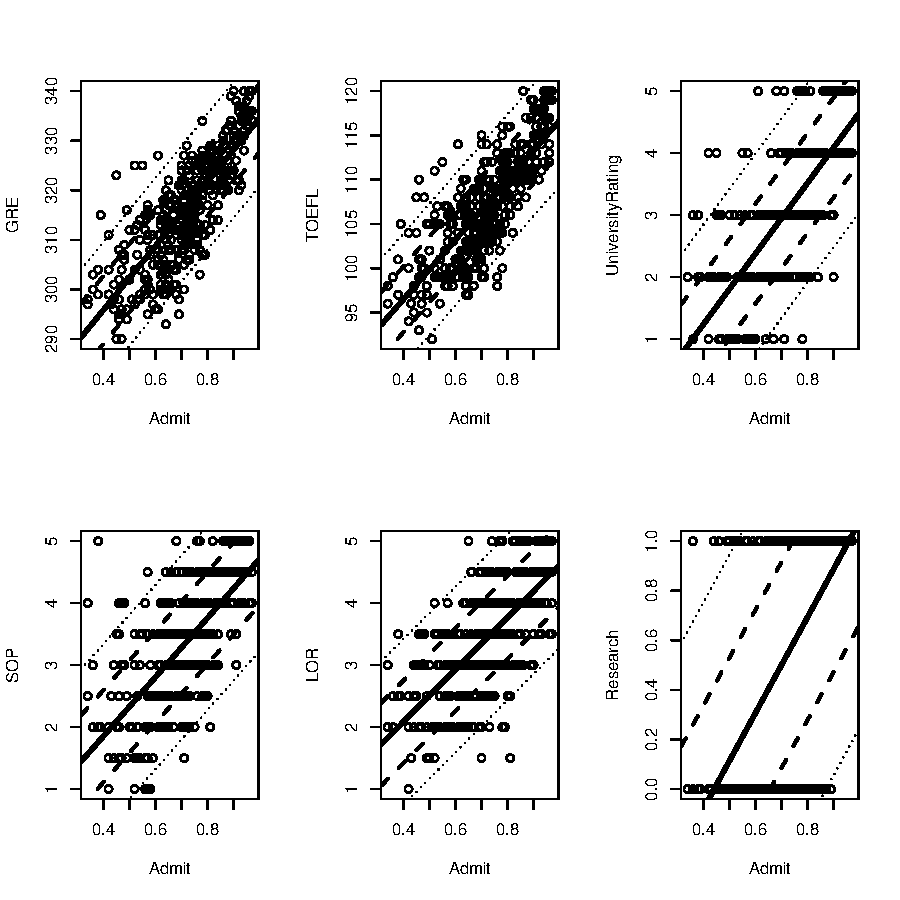
\includegraphics{entrega-analisis_grades_plot_1}
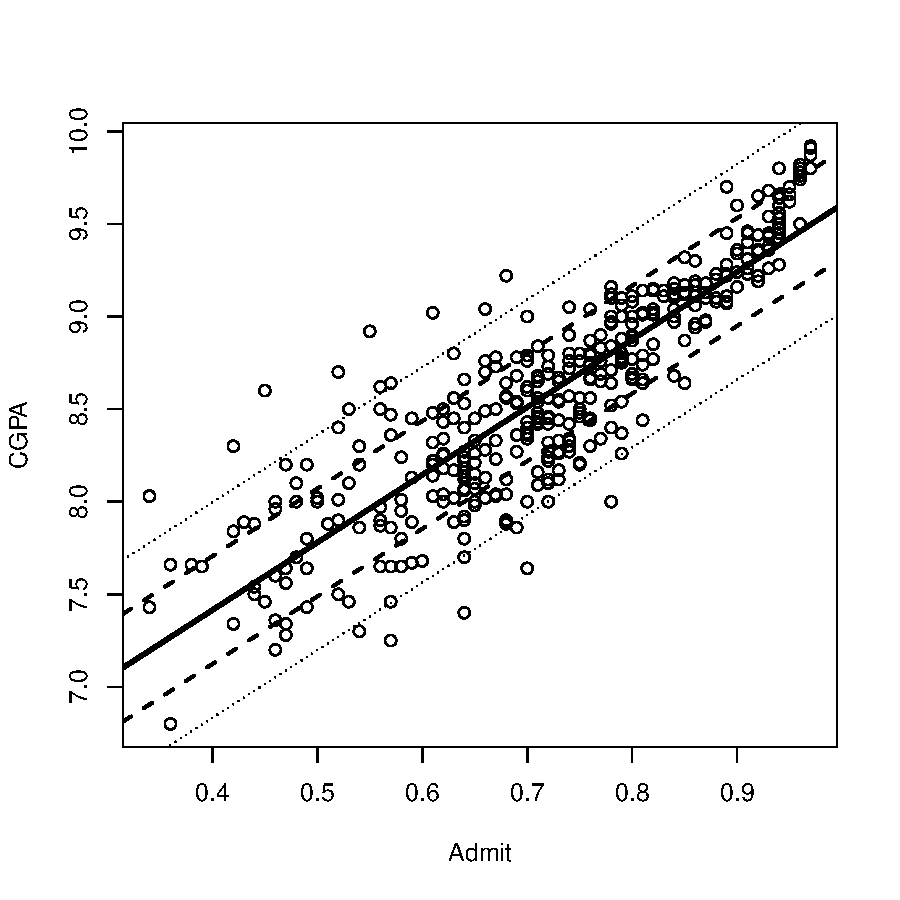
\includegraphics{entrega-analisis_grades_plot_2}
\end{center}
Vemos como en la nota media la recta de regresión se ajusta muy bien a los datos que se tienen.

%------------------------------------------------------------------------------------------------------------------------------------------------------------------------
\newpage
\section{Funciones implementadas por nosotros}
\subsection{Tomadas de la práctica 1}
\begin{Schunk}
\begin{Sinput}
> mediaAritmetica
\end{Sinput}
\begin{Soutput}
function(data){
  acc <- 0
  for (value in data) {
    acc <- acc + value
  }
  acc / length(data)
}
<bytecode: 0x7fd1ae42f338>
\end{Soutput}
\begin{Sinput}
> varianza
\end{Sinput}
\begin{Soutput}
function(data) {
  v_media <- mediaAritmetica(data)
  acc = 0
  for (value in data){
    acc <- acc + (value - v_media)^2
  }
  acc/length(data)
}
<bytecode: 0x7fd1aed427f8>
\end{Soutput}
\begin{Sinput}
> desviacionTipica
\end{Sinput}
\begin{Soutput}
function (data) {
  varianza(data)^(1/2)
}
\end{Soutput}
\end{Schunk}
\subsection{Para el anális de regresión}
\begin{Schunk}
\begin{Sinput}
> covarianza
\end{Sinput}
\begin{Soutput}
function(x, y) {
  media_x <- mediaAritmetica(x)
  media_y <- mediaAritmetica(y)
  len <- min(length(x), length(y))
  acc <- 0
  for (i in 1:len) {
    acc <- acc + x[i] * y[i]
  }
  acc/len - media_x*media_y
}
<bytecode: 0x7fd1b0956d80>
\end{Soutput}
\begin{Sinput}
> correlacion
\end{Sinput}
\begin{Soutput}
function(x, y) {
  covarianza_ <- covarianza(x, y)
  desviacion_tipica_x <- desviacionTipica(x)
  desviacion_tipica_y <- desviacionTipica(y)
  covarianza_/(desviacion_tipica_x*desviacion_tipica_y)
}
\end{Soutput}
\begin{Sinput}
> SSR
\end{Sinput}
\begin{Soutput}
function (x, y, regresion){
  media_y <- mediaAritmetica(y)
  acc <- 0
  for (value in x){
    acc <- acc + ((regresion$coefficients[2]*value+regresion$coefficients[1]) - media_y)^2
  }
  acc
}
<bytecode: 0x7fd1b20e6378>
\end{Soutput}
\begin{Sinput}
> SSY
\end{Sinput}
\begin{Soutput}
function (y, regresion){
  media_y <- mediaAritmetica(y)
  acc <- 0
  for (value in y){
    acc <- acc + (value - media_y)^2
  }
  acc
}
<bytecode: 0x7fd1b3518800>
\end{Soutput}
\begin{Sinput}
> correlacionCuadrada
\end{Sinput}
\begin{Soutput}
function (x, y ,regresion){
  SSR(x, y ,regresion) / SSY(y ,regresion)
}
<bytecode: 0x7fd1b2083bc0>
\end{Soutput}
\begin{Sinput}
> errorEstandar
\end{Sinput}
\begin{Soutput}
function (x, y, regresion) {
  len <- min(length(x), length(y))
  acc <- 0
  for (i in 1:len){
    acc <- acc + (y[i] - (regresion2$coefficients[2]*x[i]+regresion2$coefficients[1]))^2
  }
  sqrt(acc/(len))
}
<bytecode: 0x7fd1af103380>
\end{Soutput}
\begin{Sinput}
> regLine
\end{Sinput}
\begin{Soutput}
function (x, y) {
  covarianza_ <- covarianza (x, y)
  varianza_ <- varianza (x)
  media_x <- mediaAritmetica(x)
  media_y <- mediaAritmetica(y)
  a <- covarianza_/varianza_
  b <- media_y - a * media_x
  data.frame(coefficients=c(b, a))
}
<bytecode: 0x7fd1b30caf20>
\end{Soutput}
\begin{Sinput}
> regPlot
\end{Sinput}
\begin{Soutput}
function (x, y, regresion, xlabel="", ylabel="") {
  plot(x, y, xlab=xlabel, ylab=ylabel)
  reg95up <- regresion
  reg95up$coefficients[1] = reg95up$coefficients[1] + 2*summary(regresion)$sigma
  reg66up <- regresion
  reg66up$coefficients[1] = reg66up$coefficients[1] + summary(regresion)$sigma
  reg66down <- regresion
  reg66down$coefficients[1] = reg66down$coefficients[1] - summary(regresion)$sigma
  reg95down <- regresion
  reg95down$coefficients[1] = reg95down$coefficients[1] - 2*summary(regresion)$sigma
  abline(reg95up, "gray", lty=3, lwd=1)
  abline(reg66up, "gray", lty=2, lwd=2)
  abline(regresion, "black", lty=1, lwd=3)
  abline(reg66down, "gray", lty=2, lwd=2)
  abline(reg95down, "gray", lty=3, lwd=1)
}
<bytecode: 0x7fd1b3809e70>
\end{Soutput}
\end{Schunk}
\end{document}
